S\documentclass[preprint,12pt]{elsarticle}
\usepackage{graphicx}
\usepackage{amssymb}
\usepackage{amsmath}
\usepackage{lineno}
\usepackage{booktabs}
\usepackage{hyperref}
\usepackage{cleveref}
\journal{Journal Name}

\begin{document}
\begin{frontmatter}
%% Title, authors and addresses

\title{A Mathematical model for Thelaziasis}

\author{Acu\~na Zegarra M. A., Diaz-Infante Velasco S., Olmos Liceaga D.}
\address{Universidad de Sonora}
\begin{abstract}
%% Text of abstract
In the present manuscript we present a mathematical model for thelaziasis in cattle. 
By appliyng different type of controls, we find optimal strategies to reduce the endemic levels.
\end{abstract}

\begin{keyword}
Thelaziasis \sep Mathematical Model \sep Parameter Estimation \sep Basic Reproductive number
%% keywords here, in the form: keyword \sep keyword

%% MSC codes here, in the form: \MSC code \sep code
%% or \MSC[2008] code \sep code (2000 is the default)

\end{keyword}

\end{frontmatter}

%%
%% Start line numbering here if you want
%%
\linenumbers

%% main text
\section{Introduction}
\label{Section:Intro}

\noindent Thelaziasis is a vector neglected disease that affects mainly mammals, including humans and in a minor scales, birds. In humans, even it has been found in rare cases through the world, it has a higher presence in several areas of Asia, where it occurs in rural areas with high levels of poverty, and where the main hosts are children and the elderly \cite{Wang:2014,Zhang:2017,Krishnachary:2014}. The presence of these worms in its final hosts might result in excesive lacrimation, conjuntivitis, keratitis, epiphora and corneal ulcers \cite{Asrat:2016}, but in humans also can be cause of ocular morbidity \cite{Krishnachary:2014}.

\noindent Transmission takes place due to the presence of a vector, which are usually flies and they act as intermediate hosts \cite{Otranto:2003_2}. Flies have a life expectancy of about 28 days, but it might live up to two months (\cite{sanchez:1998}). The first larval stage (L1) of the worm is ingested by the fly when it feeds from lachrymal secretions, where in the internal organs, the worm develops into its second (L2) and third (L3) larval stages within 21 days post infection \cite{Otranto:2003}. Other studies \cite{Chanie:2014}, show that flies infected with \textit{Thelazia lacrymalis} can reach the infective stage in 12-15 days, while this takes 28-32 days for flies infected with \textit{T. gulosa} \cite{Chanie:2014}. Once in the infective stage, the fly releases L3 larvae into the definite host. Finally, once in the definite host, the L3 larvae matures within 3 to 6 weeks, where the new worm deposits new eggs into the definite host becoming infective \cite{Chanie:2014}. Foxes lifespan is 2 years \cite{Devenish:2014}.


\noindent The transmission depends upon the presence of vectors and therefore thelaziasis has a seasonal occurrence \cite{Asrat:2016}. In this work we focus on the control of the disease which occurs in one year season only.

\noindent A proper understanding in the control of thelaziasis in animals can be of great interest so to prevent possible future outbreaks in animals or humans. Control strategies for thelaziasis include treatment of infected individuals. Dog thelaziasis has been treated with a topical formulation of $10\%$ imidacloprid and $2.5\%$ moxidectin \cite{Bianciardi:2005},


In \cite{shen:2006}, the authors comment control strategies to treat human thelaziosis.




%which may vary depending on the regions where thelaziasis is present. For example, in Europe \textit{Thelazia Callipaeda} is transmitted by male fruitflies \textit{Phortica variegata} \cite{Palfreyman:2018}. 

%\noindent The transmitted by the face fly \cite{Otranto:2003}. The disease has spread in animals but in humans it has been reported but in a very isolated cases \cite{Wang:2014}, \cite{Otranto:2008}, \cite{shen:2006}.\\

\noindent In \cite{Moolenbeek:1980} it was found the presence of \textit{Thelazia gulosa} and \textit{Thelazia lacrymalis} in cattle where the main responsible vector is the face fly (\textit{Musca autumnalis}) in which of larvae of \textit{Thelaszia spp} were found. Data from slaugtered cattle was collected from April to October 1978. In \cite{Lyons:2000} the authors present a survey for different diseases in equids in Kentucky USA. In their study, they found the presence \textit{Thelazia Lacrymalis} in which it is pressumed that the face fly (\textit{Musca autumnalis}) is the vector responsible for transmission. Otranto et. al. \cite{Otranto:2003} made a survey in different regions in Italy to observe the current status on dogs, cats and foxes. In their work they present the proportion of infected animals (by \textit{Thelazia Callipaeda}) in each of the regions they studied. In \cite{Dubay:2000} data about the proportions of mule deer from Wyoming and Utah by \textit{T. californiensis} was reported. Asrat \cite{Asrat:2016} sudy the prevalence of Thelaziasis in Ethiopia whereas Beitel \cite{Beitel:1974} studied the prevalence of eyeworms in the columbian black tailed deer in Oregon, USA by \textit{Thelazia californiensis}. Khedri et. al. \cite{Khedri:2016} present a one year data about infected bovine in Southeast Iran (puede ser útil).

\noindent In \cite{Ohara:1989}, the authors present a study about the prevalence and intensity of \textit{Thelazia spp} in a flies population in Alberta, Canada.


In \cite{Beitel:1974} studied the prevalence of eyeworms in the Columbian Black-Tailed Deer in Oregon. 

A special work was done in \cite{Moolenbeek:1980} were it was estimated the proportion of infected animals as well as the proportion of infected vectors.

\subsection{Some questions to explore.}
\noindent An important issue in this disease is that the propagation coincides with the presence of flies that carry the disease. If the life expectancy of the fly is reduced, then
the complete cycle of the thelazia within the vector does not complete and therefore, the 
disease no longer can be transmitted. Therefore, it might be expected that as soon as the temperature of a place of study is reduced, then the levels of the infected individuals 
with thelazia, must reach a final steady level.

\noindent In the mathematical side, analyse the model about stability, persistance, what would happen if stochasticity gets implemented? how?

\subsection{Model parameters}


\noindent We will use the model to fit two data sets. One referring to a multi-host case given by dogs and foxes and the second in a one host study, particularly the case of cattle.
%\subsubsection{Dogs and foxes}
%\noindent Foxes lifespan is about 2 years \cite{Devenish:2014}. Dogs lifespan is approximately 7 to 14 years \cite{selman:2013}.

\subsubsection{Cattle only.}
\noindent The problem can be seen as a simple host or multi-host when considering beef and milk cattle.
\noindent Some considerations about the life expectancy of the individuals. A common technique 
to detect thelazia in farming animals is done by sacrificing the animal. In this case, the infected individual is no longer part of the infection cycle and basically out of the dynamics.
In this work we consider that the sample used to observe the proportion of infected individuals is of little to neglected significance respect to the total population.

\noindent The life expectancy of beef cattle is approximately 16 to 24 months (and can be up to 30 months \cite{stanley:2003}), whereas for diary cattle is 5 to 6 years. The natural cattle life expectancy is 18 to 22 years.


\section{Mathematical Model}

\noindent Our model is based on the interaction of flies and cattle. For the model, we consider that infected cattle shows visual presence of worms. A sample of the herd is taken per time unit and the animals are revised if there is presence of worms. Then vaccination proceeds.  
Following the formulation in Esteva \cite{Esteva:1998} we obtain the 
following SI vector host model for cattle and flies.
\begin{equation}\label{Eq:SIvectorhostmodel}
\begin{aligned}
    \dot{S}_f&= 
        \Lambda_f-\frac{\beta_f}{N_c^{\infty}}I_cS_f-\mu_fS_f
    \\
    \dot{L}_f&= 
        \frac{\beta_f}{N_c^{\infty}}I_cS_f-\left(k_f+\mu_f\right)L_f
    \\
    \dot{I}_f&= 
        k_f L_f-\mu_fI_f
    \\
    \dot{S}_c&= 
        \Lambda_c-\frac{\beta_c}{N_c^{\infty}}I_fS_c-\mu_cS_c
    \\
    \dot{L}_c&= 
        \frac{\beta_c}{N_c^{\infty}}I_fS_c-\left(\mu_c+k_c\right)L_c
    \\
    \dot{I}_c&= k_c L_c-\mu_c +\delta I_c
    \\
\end{aligned}
\end{equation}

\noindent After control is applied (need to find out the models we will apply)

\begin{equation}\label{Eq:SIvectorhostmodelcontrol}
\begin{aligned}
    \dot{S}_f&= 
        \Lambda_f-\frac{\beta_f}{N_c^{\infty}}I_c S_f-(\mu_f+w(t))S_f
    \\
    \dot{L}_f&= 
        \frac{\beta_f}{N_c^{\infty}} I_c S_f-
        \left(
            k_f + w(t) + \mu_f
        \right) L_f
    \\
    \dot{I}_f&= 
        k_f L_f-(w(t)+\mu_f)I_f
    \\
    \dot{S}_c&= 
        \Lambda_c-\frac{\beta_c}{N_c^{\infty}}I_f S_c-
        \left(
            \mu_c + v(t)
        \right)
        S_c + \rho T_c
    \\
    \dot{L}_c&= 
        \frac{\beta_c}{N_c^{\infty}} I_f S_c - 
        \left(
            \mu_c + v(t) + 
            k_c
        \right)L_c
    \\
    \dot{I}_c&= 
        k_c L_c - 
        (\mu_c + v(t) + \delta u(t))I_c
    \\
    \dot{T}_c&= 
        \delta u(t) I_c - 
        \left(
            \rho  + \mu_c
        \right) T_c
    \\
\end{aligned}
\end{equation}
where $v(t)$, $u(t)$ and $w(t)$ represent culling, treatment and fumigation, respectively.\\
%where $N_c=S_c+L_c+I_c$. 
\noindent A second version of the model takes into account two different disease stages for the definite host (cows). Such stages refer to the severity of the worms parasitism. The main idea is to have different control measures depending on the severity of the disease. Therefore, we define two 
different infected classes for infected cows, $I_{cl}$ and $I_{ch}$ which refer infected cows with light and heavy worm burden, respectively. Once a vector has transmitted some larvae into some susceptible individuals they become infected and depending on the amount of deposited larvae, a fraction $\theta$ of the susceptible hosts move to the $I_{cl}$ class and the complement $1-\theta$, move to the $I_{ch}$ class. An individual in the $I_{cl}$ class might move to the $I_{ch}$ class as it keep continuously in contact with vectors which remain depositing larvae into the eyes in such way that eventually the light worm burden becomes high and then a change to the class $I_{ch}$. Our model in this case becomes
\begin{equation}\label{Eq:SIvectorhostmodel_v2}
\begin{aligned}
    \dot{S}_f&= 
        \Lambda_f-\frac{S_f}{N_c^{\infty}}\left(\beta_fI_{cl}+\tilde{\beta}_fI_{ch} \right)-\mu_fS_f
    \\
    \dot{L}_f&= 
        \frac{S_f}{N_c^{\infty}}\left(\beta_fI_{cl}+\tilde{\beta}_fI_{ch}\right)-\left(k_f+\mu_f\right)L_f
    \\
    \dot{I}_f&= 
        k_f L_f-\mu_fI_f
    \\
    \dot{S}_c&= 
        \Lambda_c-\frac{\beta_c}{N_c^{\infty}}I_fS_c-\mu_cS_c
    \\
    \dot{L}_c&= 
        \frac{\beta_c}{N_c^{\infty}}I_fS_c-\left(\mu_c+k_c\right)L_c
    \\
    \dot{I}_{cl}&=  \theta k_c L_c- \frac{\tilde{\beta}_c}{N_c^{\infty}}I_{cl}I_f-\mu_c I_{cl} 
    \\
    \dot{I}_{ch}&= (1-\theta) k_c L_c + \frac{\tilde{\beta}_c}{N_c^{\infty}}I_{cl}I_f- \mu_c I_{ch}
    \\
\end{aligned}
\end{equation}
\noindent In order to control the presence of eyeworms we focus our strategy based on \cite{Manjunath:2016}, in which there are considered three levels of worm burden. For those scenarios, the two less severe are treated with medication, whereas the most severe consist on direct removal. In our model, we focus on two generic strategies. The use of medicationine, which is applied for light to medium levels as one single class $(I_{cl})$ and removal for the heavy worm burden $(I_{ch})$. Under these hyphothesis our model with applied control becomes,  
\begin{equation}\label{Eq:SIvectorhostmodel_v2controlled}
\begin{aligned}
    \dot{S}_f&= 
        \Lambda_f-\frac{S_f}{N_c^{\infty}}\left(\beta_fI_{cl}+\tilde{\beta}_fI_{ch} \right)-\left(\mu_f+w_f(t)\right)S_f
    \\
    \dot{L}_f&= 
        \frac{S_f}{N_c^{\infty}}\left(\beta_fI_{cl}+\tilde{\beta}_fI_{ch}\right)-\left(k_f+\mu_f+w_f(t)\right)L_f
    \\
    \dot{I}_f&= 
        k_f L_f-\left(w_f(t)+\mu_f\right)I_f
    \\
    \dot{S}_c&= 
        \Lambda_c-\frac{\beta_c}{N_c^{\infty}}I_fS_c-\mu_cS_c+v_h(t)I_{ch}+\rho T_c
    \\
    \dot{L}_c&= 
        \frac{\beta_c}{N_c^{\infty}}I_fS_c-\left(\mu_c+k_c\right)L_c
    \\
    \dot{I}_{cl}&=  \theta k_c L_c- \frac{\tilde{\beta}_c}{N_c^{\infty}}I_{cl}I_f-(\mu_c+v_l(t)) I_{cl} 
    \\
    \dot{I}_{ch}&= (1-\theta) k_c L_c + \frac{\tilde{\beta}_c}{N_c^{\infty}}I_{cl}I_f- (\mu_c+v_h(t)) I_{ch}
    \\
    \dot{T}_c&= v_l(t)I_{cl}-\left(\mu_c+\rho\right)T_c
\end{aligned}
\end{equation}
where $w_f(t)$ represents fly fumigation, $v_l(t)$ is cow treatment by medication and $v_h(t)$ consists on worm removal.\\

\noindent For the uncontrolled model (System \ref{Eq:SIvectorhostmodel}), the basic reproductive number is given by
 %\begin{equation}
 %    R_0=\left(\left(\frac{k_f}{\mu_f+k_f}\right)\left(%\frac{\beta_c}{\mu_f}\right)\left(\frac{k_c}{k_c+\mu_c%}\right)\left(\frac{F_c\beta_f}{\mu_c} \right) %\right)^{1/4}
 %\end{equation}
  \begin{equation}\label{eq:R0}
     R_0=\left(\frac{\beta_c\beta_f k_c k_fN_f^{\infty}}{\mu_f(\mu_c+k_c)(\mu_c+\delta_c)(\mu_f+k_f)N_c^{\infty}} \right)^{1/4}
 \end{equation}
 
% where 
% $
%    \displaystyle
%    F_c=\frac{N_f^{\infty}}{N_c^{\infty}}
%$, 
\noindent where $
    \displaystyle
    N_f^{\infty}=\frac{\Lambda_f}{\mu_f}
    $ 
 and 
$
    \displaystyle
    N_c^{\infty} = \frac{\Lambda_c}{\mu_c}
$. Table \ref{Table:Parameters} shows 
 the meaning and values of the parameters considered in this study.
 
%Clearly, the root is due to the presence of the four-cycle as shown in figure (Z)
%which is the contribution of the infection cycles fox-flies and dogs-flies.\\

%About the number of cattle in a farm
%http://www.agr.gc.ca/eng/industry-markets-and-trade/canadian-agri-food-sector-intelligence/red-meat-and-livestock/red-meat-and-livestock-market-information/inventories/cattle-inventory-by-farm-type-ontario/?id=1415860000081

\begin{table}[htb]
	\begin{center}
        \begin{tabular}{cllc}
	%		\toprule
			\hline
			Parameter		&	Meaning & Interval & Reference
			\\
			\midrule
			$N_c$& Total number of &&\\
			&individuals at time $t$ &1000&This study
			\\
			$\Lambda_f$& Fly recruitment rate & & This study
			\\
			$\Lambda_c$& Cattle recruitment rate & & This study
			\\			
			$\beta_c$& Number of successful &&\\
			&contacts of a fly &&
				\\
			& that infects a cattle host &&This study
				\\
			$\beta_f$& Number of successful&&\\
			&contacts in which &&
				\\
			& a fly gets infected by a &&\\
			&cattle host &&This study
				\\
			$k_v^{-1}$	& average latency time &&\\
			&for vectors & 14-21 days &\cite{Otranto:bookchapter}
			\\
				& & 12-15 days &\\
				&&(\textit{T. Lacrymalis}) &\cite{Chanie:2014}
			\\
				& & 28-32 days&\\ 
				&&(\textit{T. Gulosa}) &\cite{Chanie:2014}
			\\
			$k_{i}^{-1}$
			&
				average latency time &&\\
				&for hosts $i=1,2$ & $\approx$ 35 days& \cite{Otranto:bookchapter}
			\\
			& & 21-42 days& \cite{Chanie:2014}
			\\			
			 $\mu_v^{-1}$	& vector average lifespan & 30-60 months&\cite{sanchez:1998}
			\\
			$\mu_c^{-1}$
			&
				cows average lifespan & 1080 days& \cite{FAOweb}
			\\
    		\bottomrule
		\end{tabular}
	\end{center}
	\caption{
		Parameter meaning and values.}
    \label{Table:Parameters}
\end{table}


\section{Local and global stability analysis}
\noindent In system~\ref{Eq:SIvectorhostmodel}, we observe that the equations for the total cow and fly populations are given by:
\begin{equation*}
    \begin{aligned}
        \dot{N}_{f} &= \Lambda_{f} - \mu_{f}N_{f}\\
        \dot{N}_{c} &= \Lambda_{c} - \mu_{c}N_{c},
    \end{aligned}
\end{equation*}
so it implies that, for a sufficiently large time, the fly and cow populations will tend to $\displaystyle N_f^{\infty}=\frac{\Lambda_f}{\mu_f}$ and $\displaystyle N_c^{\infty}=\frac{\Lambda_c}{\mu_c}$, respectively. In consequence, we can reduce system~\ref{Eq:SIvectorhostmodel},obtaining:
\begin{equation}\label{Eq:ReduceSIvectorhostmodel}
\begin{aligned}
    \dot{L}_f&= 
        \frac{\beta_f}{N_c^{\infty}}I_c\left(N_f^{\infty} - L_f - I_f\right)-\left(k_f+\mu_f\right)L_f
    \\
    \dot{I}_f&= 
        k_f L_f-\mu_f I_f
    \\
    \dot{S}_c&= 
        \Lambda_c-\frac{\beta_c}{N_c^{\infty}}I_fS_c-\mu_cS_c+\rho \left(N_c^{\infty} - S_c - L_c - I_c\right)
    \\
    \dot{L}_c&= 
        \frac{\beta_c}{N_c^{\infty}}I_fS_c-\left(\mu_c+k_c\right)L_c
    \\
    \dot{I}_c&= k_c L_c-\left(\mu_c +\delta\right)I_c
\end{aligned}
\end{equation}

\noindent System~\ref{Eq:ReduceSIvectorhostmodel} has two equilibrium points in $\Omega = \{\left(L_{f},I_{f},S_{c},L_{c},I_{c}\right)\in \mathbb{R}^{5}: 0\leq L_{f} + I_{f}\leq N_{f}^{\infty}, 0\leq S_{c} + L_{c} + I_{c}\leq N_{c}^{\infty}\}$. The disease free equilibrium 
$$
    S_1 = \left(L_{f1}^*,I_{f1}^*,S_{c1}^*,L_{c1}^*,I_{c1}^*\right) = 
    \left(0,0,\frac{\Lambda_c}{\mu_c},0,0\right)
$$ 
and the endemic equilibrium 
$$
    S_2 = (L_{f2}^*,I_{f2}^*,S_{c2}^*,L_{c2}^*,I_{c2}^*) = 
    .
$$

\noindent Theorem. The disease free equilibrium point $S_1$ is globally asymptotically stable in $\Omega$, if $R_0<1$.\\
Proof: Consider the Lyapunov function
$$V(L_f,I_f,S_c,L_c,I_c) = a_1\left(S_c - N_{c}^{\infty} - N_{c}^{\infty}\ln{\frac{S_c}{N_{c}^{\infty}}}\right) + a_2 L_f + I_f + a_3 L_c + a_4 I_c~,$$
with
$$
a_1 = a_2 = \frac{k_c}{\mu_c + k_c},\ a_3 = \left(\frac{k_f}{\mu_f + k_f}\right)\left(\frac{k_c}{\mu_c + k_c}\right)\frac{\beta_c}{\mu_f},\ a_4 = \left(\frac{k_c}{\mu_c + k_c}\right)\frac{\beta_c}{\mu_f}~.
$$
The derivative of $V$ is as follows:
\begin{equation}\label{Eq:DFE_Lyapunov}
    \begin{aligned}
    \dot{V} &= a_1\left(1 - \frac{N_{c}^{\infty}}{S_c}\right)\left[\Lambda_c-\frac{\beta_c}{N_c^{\infty}}I_fS_c-\mu_cS_c+\rho \left(N_c^{\infty} - S_c - L_c - I_c\right)\right]\\
    &\quad + a_2 \left[\frac{\beta_c}{N_c^{\infty}}I_fS_c-\left(\mu_c+k_c\right)L_c\right] + \left[k_c L_c-\left(\mu_c +\delta\right)I_c\right]\\
    &\quad + a_3\left[\frac{\beta_f}{N_c^{\infty}}I_c\left(N_f^{\infty} - L_f - I_f\right)-\left(k_f+\mu_f\right)L_f\right] + a_4 \left[k_f L_f-\mu_f I_f \right]
    \end{aligned}
\end{equation}
Substituting the values of $a_1$, $a_2$, $a_3$ and $a_4$, we simplify equation~\ref{Eq:DFE_Lyapunov},
\begin{equation*}
    \begin{aligned}
    \dot{V} &= -a_1\frac{\left(S_c - N_{c}^{\infty}\right)^{2}}{S_c} - a_1\rho\left(N_{c}^{\infty} - S_c - I_c - L_c\right)\left(\frac{N_{c}^{\infty} - S_c}{S_c}\right)\\
    &\quad\ - a_3\beta_f\frac{I_c}{N_{c}^{\infty}}\left(L_f + I_f\right) - \left(\mu_c + k_c\right)\left[1 - \frac{\beta_c\beta_f k_c k_fN_f^{\infty}}{\mu_f(\mu_c+k_c)(\mu_c+\delta_c)(\mu_f+k_f)N_c^{\infty}}\right]I_c
    \end{aligned}
\end{equation*}
Replacing the expression for $\mathcal{R}_{0}$ given in~\eqref{eq:R0}, we conclude that $\dot{V} < 0$ for $\mathcal{R}_{0} < 1$. Finally, as $S_{1}$ is the only invariant set in $\Omega$ such that $\dot{V}=0$, from the La Salle-Lyapunov theorem, it follows that if $\mathcal{R}_{0} < 1$, then $S_{1}$ is globally asymptotically stable in $\Omega$.

\noindent Theorem. A unique endemic equilibrium exists when $R_0>1$.\\
Proof: Solving the equations for the state variables, we end up with the following relationships\\
$S_f=\frac{\Lambda_f}{\left(\frac{\beta_f}{N_c^{\infty}}I_c+\mu_f\right)}$;
$L_f=\left(\frac{\beta_f}{N_c^{\infty}(\lambda_f+\mu_f)}\right)\left(\frac{\Lambda_f}{\left(\frac{\beta_f}{N_c^{\infty}}I_c+\mu_f\right)}\right)I_c$;\\
$I_f=\left(\frac{\lambda_f}{\mu_f}\right)\left(\frac{\beta_f}{N_c^{\infty}(\lambda_f+\mu_f)}\right)\left(\frac{\Lambda_f}{\left(\frac{\beta_f}{N_c^{\infty}}I_c+\mu_f\right)}\right)I_c$;
$S_c=\frac{(\mu_c+\lambda_c)(\mu_c+\delta)(\lambda_f+\mu_f)\mu_fN_c^{\infty}^2\left(\frac{\beta_f}{N_c^{\infty}}I_c+\mu_f\right)}{\lambda_c\beta_c\lambda_f\beta_f\Lambda_f}$;\\
$T_c=\frac{\delta T_c}{\rho+\mu_c}$;
$L_c=\frac{(\mu_c+\delta)I_c}{\lambda_c}$ and
$I_c=\frac{A}{B}\left(R_0^4-1\right)$,
with\\
$A=\frac{\mu_c\mu_f^2(\mu_c+\lambda_c)(\mu_c+\delta)(\lambda_f+\mu_f)N_c^{\infty}^2}{\lambda_c\beta_c\lambda_f\beta_f\Lambda_f}$ and $B=\frac{(\mu_c+\lambda_c)(\mu_c+\delta)}{\lambda_c}\left[1+{\frac{\mu_c(\lambda_f+\mu_f)\mu_cN_c^{\infty}}{\beta_c}}\right]-\frac{\rho\delta}{\rho+\mu_c}$.\\
Clearly, $\frac{(\mu_c+\lambda_c)(\mu_c+\delta)}{\lambda_c}>\delta$, $1+{\frac{\mu_c(\lambda_f+\mu_f)\mu_c N_c^{\infty}}{\beta_c}}>1$ and $\frac{\rho\delta}{\rho+\mu_c}<\delta$. Therefore, $I_c>0$ if and only if $R_0>1$.\\

\noindent Observe that the endemic equilibrium is preserved when no control is applied into the model ($\rho=\delta=0$). For this particular case it is possible to show global stability for the endemic equilibrium\\

\noindent Theorem. The endemic equilibrium for the model with no control ($\rho=\delta=0$) is asymptotically globally stable.\\
Proof: Following the ideas in \cite{Zhou:2014}, we consider the Lyapunov function
$$V=\sum_{i=1}^6a_i\left(X_i-\overline{X}_i\ln{\frac{X_i}{\overline{X}_i}}\right),$$ where $X_i$ are the components of the vector $(S_f,L_f,I_f,S_c,L_c,I_c)$ and $\overline{X}=(\overline{S}_f,\overline{L}_f,\overline{I}_f,\overline{S}_c,\overline{L}_c,\overline{I}_c)$ are the coordinates of the endemic equilibrium. 

\noindent At the endemic equilibrium point, the following equalities hold
$$\Lambda_f=\frac{\beta_f\overline{S}_f\overline{I}_c}{N_c^{\infty}}+\mu_f\overline{S}_f \qquad \Lambda_c=\frac{\beta_c\overline{S}_c\overline{I}_f}{N_c^{\infty}}+\mu_c\overline{S}_c \qquad \mu_f+k_f=\frac{\beta_f\overline{S}_f\overline{I}_c}{N_c^{\infty}\overline{L}_f}$$
\begin{equation}\label{endemic_equalities}
\mu_c+k_c=\frac{\beta_c\overline{S}_c\overline{I}_f}{N_c^{\infty}\overline{L}_c} \qquad \mu_f=k_f\frac{\overline{L}_f}{\overline{I}_f} \qquad \mu_c= k_c\frac{\overline{L}_c}{\overline{I}_c}
\end{equation}

\noindent From this information, we obtain 
$$\dot{V}(t)=a_1\left(\Lambda_f-\frac{\beta_f}{N_c^{\infty}}I_cS_f-\mu_fS_f\right)\left(1-\frac{\overline{S}_f}{S_f}\right)+a_2\left(\frac{\beta_f}{N_c^{\infty}}I_cS_f-\left(k_f+\mu_f\right)L_f\right)\left(1-\frac{\overline{L}_f}{L_f}\right)$$
$$+a_3\left(k_f L_f-\mu_fI_f\right)\left(1-\frac{\overline{I}_f}{I_f}\right)+a_4\left(\Lambda_c-\frac{\beta_c}{N_c^{\infty}}I_fS_c-\mu_cS_c\right)\left(1-\frac{\overline{S}_c}{S_c}\right)$$
$$+a_5\left(\frac{\beta_c}{N_c^{\infty}}I_fS_c-\left(\mu_c+k_c\right)L_c\right)\left(1-\frac{\overline{L}_c}{L_c}\right)+a_6\left(k_c L_c-\mu_cI_c\right)\left(1-\frac{\overline{I}_c}{I_c}\right).$$

\noindent Then, by taking the scaled variables
$$
s_f^*=\frac{S_f}{\overline{S}_f};\quad l_f^*=\frac{L_f}{\overline{L}_f};\quad i_f^*=\frac{I_f}{\overline{I}_f};\quad
s_c^*=\frac{S_c}{\overline{S}_c};\quad l_c^*=\frac{L_c}{\overline{L}_c};\quad i_c^*=\frac{I_c}{\overline{I}_c}
$$
and the use of the equalities in \ref{endemic_equalities}, our last expression becomes
$$\dot{V}(t)=-a_1\frac{\mu_f\overline{S}_f}{s_f^*}\left(s_f^*-1\right)^2-a_4\frac{\mu_c\overline{S}_c}{s_c^*}\left(s_c^*-1\right)^2+a_1\frac{\beta_f\overline{S}_f\overline{I}_c}{N_c^{\infty}}(1-s_f^*i_c^*)-a_1\frac{\beta_f\overline{S}_f\overline{I}_c}{s_f^*N_c^{\infty}}(1-s_f^*i_c^*)$$
$$+a_2\frac{\beta_f\overline{S}_f\overline{I}_c}{N_c^{\infty}}\left(s_f^*i_c^*-l_f^*\right)\left(1-\frac{1}{l_f^*}\right)+a_3k_f\overline{L}_f\left(1-\frac{1}{i_f^*}\right)\left(l_f^*-i_f^*\right)$$
$$+a_4\frac{\beta_c\overline{S}_c\overline{I}_f}{N_c^{\infty}}\left(1-\frac{1}{s_c^*}\right)\left(1-i_f^*s_c^*\right)+a_5\frac{\beta_c\overline{S}_c\overline{I}_f}{N_c^{\infty}}\left(1-\frac{1}{l_c^*}\right)\left(i_f^*s_c^*-l_c^*\right)$$
$$+a_6k_c\overline{L}_c\left(1-\frac{1}{i_c^*}\right)\left(l_c^*-i_c^*\right).$$
After rearranging terms we end up with
$$\dot{V}(t)=-a_1\frac{\mu_f\overline{S}_f}{s_f^*}\left(s_f^*-1\right)^2-a_4\frac{\mu_c\overline{S}_c}{s_c^*}\left(s_c^*-1\right)^2+\left(a_3k_f\overline{L}_f-a_2\frac{\beta_f\overline{S}_f\overline{I}_c}{N_c^{\infty}}\right)l_f^*$$ 
$$+\left(a_4\frac{\beta_c\overline{S}_c\overline{I}_f}{N_c^{\infty}}-a_3k_f\overline{L}_f\right)i_f^*+\left(a_6k_c\overline{L}_c-a_5\frac{\beta_c\overline{I}_f\overline{S}_c}{N_c^{\infty}}\right)l_c^*+\left(a_1\frac{\beta_f\overline{S}_f\overline{I}_c}{N_c^{\infty}}-a_6k_c\overline{L}_c\right)i_c^*$$
$$+\left(a_2-a_1\right)\frac{\beta_f\overline{S}_f\overline{I}_c}{N_c^{\infty}}s_f^*i_c^*+\left(a_5-a_4\right)\frac{\beta_c\overline{S}_c\overline{I}_f}{N_c^{\infty}}i_f^*s_c^*+a_1\frac{\beta_f\overline{S}_f\overline{I}_c}{N_c^{\infty}}+a_2\frac{\beta_f\overline{S}_f\overline{I}_c}{N_c^{\infty}}$$
$$+a_3k_f\overline{L}_f+a_4\frac{\beta_c\overline{S}_c\overline{I}_f}{N_c^{\infty}}+a_5\frac{\beta_c\overline{S}_c\overline{I}_f}{N_c^{\infty}}+a_6k_c\overline{L}_c-a_1\frac{\beta_f\overline{S}_f\overline{I}_c}{N_c^{\infty}}\left(\frac{1}{s_f^*}\right)-a_2\frac{\beta_f\overline{S}_f\overline{I}_c}{N_c^{\infty}}\left(\frac{s_f^*i_c^*}{l_f^*}\right)$$
$$-a_3k_f\overline{L}_f\left(\frac{l_f^*}{i_f^*}\right)-a_4\frac{\beta_c\overline{S}_c\overline{I}_f}{N_c^{\infty}}\left(\frac{1}{s_c^*}\right)-a_5\frac{\beta_c\overline{S}_c\overline{I}_f}{N_c^{\infty}}\left(\frac{s_c^*i_f^*}{l_c^*}\right)-a_6k_c\overline{L}_c\left(\frac{l_c^*}{i_c^*}\right) $$

\noindent By taking the constant values as
$$a_2=a_1;\quad a_3=\frac{\beta_f\overline{I}_c\overline{S}_f}{k_f\overline{L}_f N_c^{\infty}}a_1;\quad a_4=\frac{\beta_f\overline{I}_c\overline{S}_f}{\beta_c\overline{I}_f\overline{S}_c}a_1;\quad a_5=a_4;\quad a_6=\frac{\beta_f\overline{I}_c\overline{S}_f}{k_c\overline{L}_c N_c^{\infty}}a_1 $$,
we obtain
$$\dot{V}= -a_1\frac{\mu_f\overline{S}_f}{s_f^*}\left(s_f^*-1\right)^2-a_4\frac{\mu_c\overline{S}_c}{s_c^*}\left(s_c^*-1\right)^2+a_1\frac{\beta_f\overline{S}_f\overline{I}_c}{N_c^{\infty}}\left[6-\left(\frac{1}{s_f^*}+\frac{s_f^*i_c^*}{l_f^*}+\frac{l_f^*}{i_f^*}+\frac{1}{s_c^*}+\frac{i_f^*s_c^*}{l_c^*}+\frac{l_c^*}{i_c^*}\right)\right]$$
Now, because the arithmetic mean is larger than the geometric mean, implies that  $\frac{1}{6}\left(\frac{1}{s_f^*}+\frac{s_f^*i_c^*}{l_f^*}+\frac{l_f^*}{i_f^*}+\frac{1}{s_c^*}+\frac{i_f^*s_c^*}{l_c^*}+\frac{l_c^*}{i_c^*}\right)\geq 1$, and therefore $\dot{V}\leq 0$. Clearly, $\dot{V} = 0$ only at the endemic equilibrium.


\subsection{Persistance}

\section{Discussion}

\section{Numerical Results}

    \begin{figure*}
    \centering
    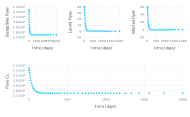
\includegraphics[width=\linewidth, keepaspectratio]{%
    Figures/flyes_disease_dynamics}
    \caption{Solution with parameters according to $R_0 < 1$.}
    \label{fig:flyesdiseasedynamics}
\end{figure*}
%
%
%
\begin{figure*}
    \centering
    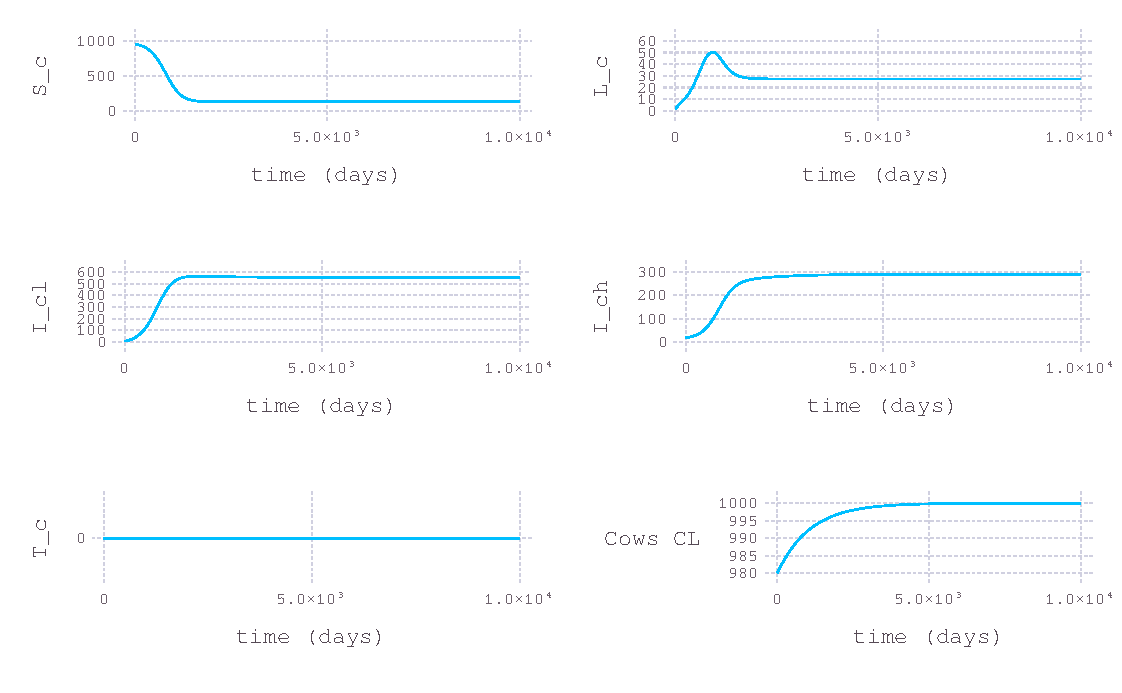
\includegraphics[width=\linewidth, keepaspectratio]{%
    Figures/cows_disease_dynamics}
    \caption{Solution with parameters according to $R_0 < 1$ 
    }
    \label{fig:cowsdiseasedynamics}
\end{figure*}


\textbf{Bibliography}
\bibliographystyle{model1-num-names}
\bibliography{thelazbiblio.bib}
\end{document}
